\documentclass[12pt,a4paper]{amsart}
\usepackage{microtype}
\usepackage[margin=2.54cm]{geometry}
%\usepackage[T2A]{fontenc}
%\usepackage[utf8]{inputenc}
%\usepackage[russian,english]{babel}
\usepackage{hyphenat}
%\usepackage[T1]{fontenc}
\usepackage{lmodern}
%\usepackage[outer]{showlabels}
\usepackage{amsfonts}
\usepackage{epsfig}
\usepackage{graphicx}
\usepackage{breqn}
\usepackage{amsmath}
\usepackage{amssymb}
\usepackage{latexsym}
\usepackage{rotating}
\usepackage{pstricks, pst-node, pst-text, pst-3d}
\usepackage{amsbsy}
\usepackage{subfig}
%\usepackage{enumerate}
%\usepackage[shortlabels]{enumitem}
%\usepackage{amsthm}
\usepackage{mathrsfs}
%\usepackage[all]{xy}
\usepackage{hyperref}
\usepackage{textcomp}
\usepackage{color}
\usepackage{verbatim}
\usepackage{subfig}
%\usepackage{biblatex}
\usepackage{afterpage}
\usepackage{pdflscape}
\usepackage{rotating}
\usepackage[super]{nth}
\usepackage{nag}
\usepackage{enumitem}
\usepackage{rotating}
\usepackage{mathtools}
\usepackage{mdframed}
\usepackage{lipsum}

\usepackage{listings}[language=Python] 
\lstset{
  basicstyle=\ttfamily,
  columns=fullflexible,
  %frame=single,
  breaklines=true,
  postbreak=\mbox{\textcolor{red}{$\hookrightarrow$}\space},
  keepspaces=true
  breakatwhitespace=true
}

\numberwithin{equation}{section}
\graphicspath{{../}}
%\graphicspath{ {./../} }

\allowdisplaybreaks[1]

\newtheorem{theorem}{Theorem}
\newtheorem{proposition}{Proposition}
\newtheorem{corollary}{Corollary}
\newtheorem{lemma}{Lemma}
\newtheorem{question}{Question}

\newtheorem{definition}{Definition}
\newtheorem{remark}{Remark}


\theoremstyle{remark}
\newtheorem{example}{Example}
\newtheorem{problem}{Problem}
\newtheorem{solution}{Solution}

\newtheorem{details}{Details}

%\newmdtheoremenv{theo}{Theorem}
%\newmdtheoremenv{details}{Details}
%\newenvironment{fdetails}
%  {\begin{mdframed}\begin{theo}}
%  {\end{theo}\end{mdframed}}

%\usepackage{framed} % or, "mdframed"
%\usepackage[framed]{ntheorem}
%\newframedtheorem{details}{Details}


%\author{Alexey Tochin}
\begin{document}
\title{Batch size vs Momentum}
\maketitle

Imagine we've pinpointed the optimal learning rate and other hyperparameters
for a gradient descent method and a specific model.
The natural progression is to train this model on more powerful hardware,
equipped with additional GPU units and RAM, enabling larger batch sizes.
But how do we adjust the gradient descent hyperparameters
to scale up effectively without disrupting the current settings?

In this article,
we explore this question along with some related ones.
Our main thesis:
\emph{changing the batch size is roughly equivalent to adjusting the learning rate and momentum.}

%In particular, we consider a reparametrization of the hyperparameter set 
%$\{$batch size,
%learning rate,
%momentum, ...$\}$
%such that the batch size can be spitted out from the fine hyperparameter fine tune.


%\section{Introduction}
%
%It is a common recommendation to increase the batch size as much as possible in order to 
%have maximal benefits from the parallelism. 
%However,
%
%1. For not small enough learning rate, the batch size grows may cause instability.
%We do not consider this phenomenon here. 
%Instead we focus on the situations of heavy model. That is the bigger batch size is limited form above
%by hardware.
%
%2. Smaller batch size may reduce overfit thanks to larger random fluctuations that approximates 
%Bayesian inference. This important topic is also not touched in the present text. 
%Considered below as exaples models do not suffer from essential overfit.
%
%We look first for a reasonable stochastic gradient descent hyperparameter parameterization.
%But before that we have to set up some notations.


\section{Notation}

Let
$\boldsymbol\theta \in \mathbb{R}^D$
be a trainable weight vector in the $D$-dimensional space of the model's trainable weights.
We denote the sequence of weight updates during the training process by
$\{\boldsymbol\theta_n\}_{n = 0,1,2,3,\ldots}$.

Let
$L(x, y; \boldsymbol\theta)$
be the loss function for a supervised model with weight
$\boldsymbol\theta$,
and a single data sample with feature
$x$
and label
$y$.
Define the loss gradient at point
$\boldsymbol\theta$
for sample
$(x_i,y_i)$
with ordering number
$i=0,1,2,\ldots$
as
$$
	\mathbf{g}_i(\boldsymbol\theta) :=
	\frac{\partial}{\partial \boldsymbol\theta} L(x_i, y_i; \boldsymbol\theta).
$$

The samples
$\{(x_i,y_i)\}_{i=0,1,2,\ldots}$
are combined into batches.
We consider the case of a fixed batch size
$b=1,2,3,\ldots$.
We define an integer-valued function
$$
	t:\quad \{0,1,2,\ldots\} \quad \rightarrow \quad \{0,1,2,\ldots\}
$$
that maps the ordering number of each sample to the ordering number of the batch it belongs to.
For example, for
$b=3$,
we have
$$
	t_0 = 0,~t_1 = 0,~t_2 = 0,~t_3 = 1,~t_4 = 1,~t_5 = 1,~t_6 = 2,~t_7 = 2,~t_8 = 2,~\dotso.
$$


\section{Learning Rate Normalization}

We begin with the simplest version of stochastic gradient descent without momentum,
parameterized by the learning rate
$\lambda^{\text{cl}} > 0$.
The weight update rule is
\begin{equation}
	\boldsymbol\theta_{n-1}~ \rightarrow~ \boldsymbol\theta_n :=
	\boldsymbol\theta_{n-1} - \lambda^{\text{cl}} \, b^{-1} \sum_{i:~ t(i) = n} \mathbf{g}_i(\boldsymbol\theta_n),
	\label{Formula: classic SGD without momentum}
\end{equation}
where
$\sum_{i:~ t(i) = n}~\dotso$
is a sum over the minibatch
$n$.
The upper index
``$~^{\text{cl}}$''
denotes the ``classically normalized'' hyperparameter normalization that we are going to reconsider.

Suppose the batch size
$b$
has changed. Our goal is to scale up
$\lambda^{\text{cl}}$
such that the shift of the weight sequence
$\{\boldsymbol\theta_n\}_{n = 0,1,2,3,\ldots}$
is minimized.
More precisely,
after the batch size change
$b \rightarrow \tilde b$,
each of the weights
$\tilde{\boldsymbol\theta}_{\tilde t(i)}$
from the new sequence should be close to the original ones
$\boldsymbol\theta_{t(i)}$
for each $i=0,1,2,\ldots$,
where $\tilde t$ corresponds to the new batch size
$\tilde b$.
It is straightforward to observe that a reasonable learning rate update is
$$
	\lambda^{\text{cl}} \rightarrow \tilde \lambda^{\text{cl}} =
	\frac{b}{\tilde b}\, \lambda^{\text{cl}}.
$$
In other words, the coefficient
$b^{-1}$
in
\eqref{Formula: classic SGD without momentum}
is not needed to maintain this behavior.

For example, if we increase the batch size by a factor
$k$,
the total contribution from
$k$
sequential steps is replaced by a single step with
$k$
times the number of samples.
The only difference between these sums is that in the latter case, a
ll gradients are calculated at the same weight,
whereas, for a smaller batch,
there are $k$ different but close weights corresponding to different sequential steps.

The mathematical motivation comes from the Taylor series approximation for small
$\lambda^{\text{cl}}$:
$$
	\mathbf{g}_i(\boldsymbol\theta_n) - \mathbf{g}_i(\boldsymbol\theta_{n-1}) =
	O\left(\left(\lambda^{\text{cl}} \right)^2\right),
$$
because
$$
	\boldsymbol\theta_n - \boldsymbol\theta_{n-1} = O(\lambda^{\text{cl}}).
$$

To experimentally confirm this analytical reasoning,
we consider the MNIST problem and a simple convolutional neural network.
We avoid advanced techniques such as batch normalization
to eliminate unnecessary additional effects.
\begin{details}[Model details]~
\begin{lstlisting}[language=Python]
model = tf.keras.Sequential([
    tf.keras.layers.Reshape(input_shape=(28, 28, 1), target_shape=(28, 28, 1)),
    tf.keras.layers.Conv2D(kernel_size=3, filters=12, padding='same', activation='relu'),
    tf.keras.layers.Conv2D(kernel_size=6, filters=24, padding='same', strides=2, activation='relu'),
    tf.keras.layers.Conv2D(kernel_size=6, filters=32, padding='same', strides=2, activation='relu'),
    tf.keras.layers.Flatten(),
    tf.keras.layers.Dense(units=256, activation='relu'),
    tf.keras.layers.Dropout(0.3),
    tf.keras.layers.Dense(units=10, activation=None)
])
\end{lstlisting}
The loss function is the standard classification cross-entropy.
\label{Details: mnist tou model}
\end{details}

It is practically complicated to compare the weight update sequences directly.
Instead, we consider the entire training progress and the mean loss convergence rate.
The considered model does not suffer from significant overfitting.
Thus, for simplicity, we present only the training dataset mean values below.

We experimentally verify that the convergence rate does not depend on the batch size,
provided
$\lambda$
is fixed.
See the figure below
\ref{Fig: batch size and lambda}.
\begin{figure}
	\centering
	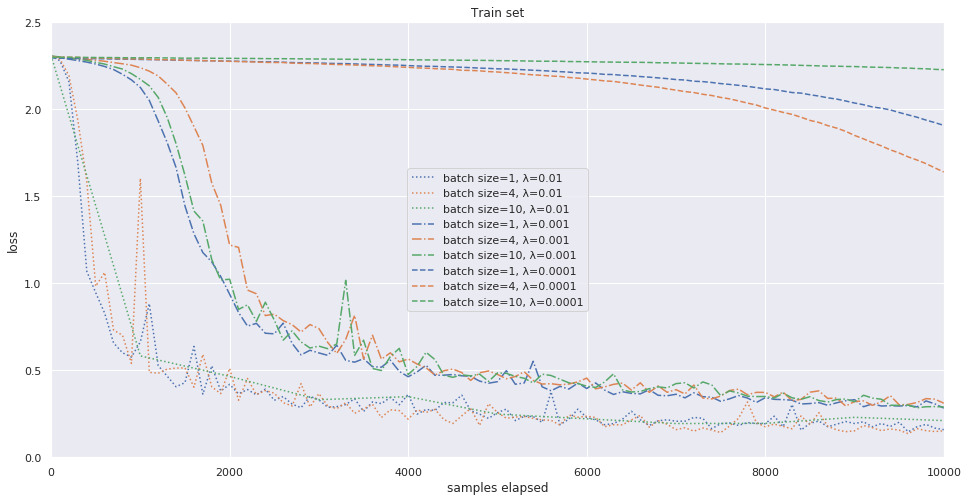
\includegraphics[width=16cm,keepaspectratio=true]{images/batch_size_and_lambda.png}
	\caption{
		Training progress evaluated on the MNIST training set
		with respect to the number of elapsed samples
		(do not confuse with update steps).
		We can observe that the convergence rate does not depend on the batch size,
		provided
		$\lambda$
		is fixed.
		On the other hand, the convergence rate, calculated in terms of the calculation cost,
		reduces dramatically for small
		$\lambda$.
	}
	\label{Fig: batch size and lambda}
\end{figure}

The speculations above motivate us to normalize the learning rate
$\lambda$
as follows:
$$
	\boldsymbol\theta_n =
	\boldsymbol\theta_{n-1} - \lambda \sum_{i:~ t(i) = n} \mathbf{g}_i(\boldsymbol\theta_n),
$$
thereby,
\begin{equation}
	\lambda^{\text{cl}} = b \, \lambda.
	\label{Formula: l^lc = b l}
\end{equation}

If the batch size
$b$
equals the entire dataset size
$N$
or is of the same order of magnitude
$b \lesssim N$,
the update on each learning step moves the weight closer to the minimum.
However, this is not the case in the mini-batch strategy when
$b \ll N$,
because each mini-batch represents very poor statistics of the entire dataset.
Mini-batch learning works due to the statistics averaging effect
after numerous learning step updates,
thanks to an aggregation of data collected from a large number of mini-batches.
This motivates the following:
\emph{
	In mini-batch learning,
	it is probably more reasonable to control the total number of samples used for the updates
	than the actual number of updates.
}

We must mention that the similarity of the training weight update sequences
at early and intermediate training stages
does not imply that the quality of the achieved minima is similar.
However, our approach also agrees with the empirical observations of
\href{https://arxiv.org/abs/1710.06451}{Samuel L. Smith and Quoc V. Le}.
It is reported there that
``...optimum batch size is proportional to the learning rate.''
In other words, there exists a batch size-independent
$\lambda$
that minimizes the final test set loss.

As mentioned in the cited paper,
a large batch size contributes to a better training set minimum.
On the other hand,
a small batch size provides additional gradient fluctuation,
improving generalization ability.
The optimal value of
$\lambda$
corresponds to a reasonable trade-off between these two effects.

Notice, however, that the speculations of this section are valid only if the convergence is stable.
It becomes unstable if the learning rate or batch size is too high.
We study this phenomenon briefly in the next section.


\section{Convergence Stability \label{Section: convergence stability}}

In this section, we experimentally investigate the stability of the neural network training process.
It is widely known that gradient descent usually becomes unstable when the learning rate exceeds
a certain value.
This is straightforward for a classical optimization problem,
where the batch equals the entire dataset.
However, instability is more complex for mini-batch training.

The results for the MNIST problem introduced above are presented in Figure
\ref{Fig: convergence stability}.

\begin{figure}
	\centering
	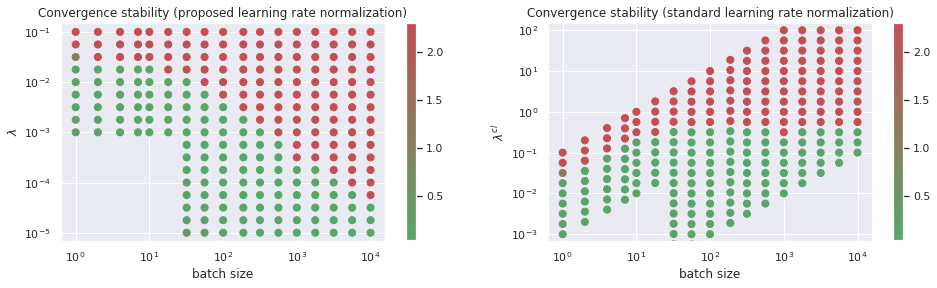
\includegraphics[width=16cm,keepaspectratio=true]{images/convergence_stability.png}
	\caption{
		Each dot corresponds to a training experiment,
		and the color denotes the loss function value on the training set a
		fter 10,000 weight updates.
		If the mean loss value is higher than
		$\log 10$,
		which corresponds to fully random classification for the 10-class MNIST problem,
		we replace it with
		$\log 10$.
		Both images are based on the same data but with different learning rate normalizations,
		see
		\eqref{Formula: l^lc = b l}.
		We can observe that the boundary between convergence and divergence modes consists
		of two approximately linear segments. Both segments correspond to some constant values of
		$\lambda$
		and
		$\lambda^{\text{cl}}$.
	}
	\label{Fig: convergence stability}
\end{figure}

Our interpretation is as follows.
There are two factors restricting stability.
The first one comes from classical optimization theory.
It is defined by the Hessian of the mean loss function
$ b^{-1} \sum_{i}{L(x_i,y_i)} $
at the minimum.
This is why we have the restriction
$\lambda^{\text{cl}} \lesssim 10^{-0.5}$.

The second restriction
$\lambda \lesssim 10^{-1.5}$
is less trivial.
It occurs when the training process is in the mini-batch mode.
This means that the batches are not statistically representative,
and the training progress is made through the accumulation of numerous steps.
Therefore, the stability of the training is defined by
$\lambda$,
which is a coefficient near the full sum of the gradients.

We do not go into more details of the stability question here.
However, we must mention that the statements from the previous section
are valid only if the training process is in the green zone of Figure
\ref{Fig: convergence stability}.


\section{Gradient Descent with Momentum \label{Section: Gradient descent with momentum}}

Next, we study the effects of equipping gradient descent with momentum.
The most widely used parameterization for this approach is as follows:
\begin{equation}
	\begin{aligned}
		\mathbf{v}^{\text{cl}}_n
			&= m^{\text{cl}}\, \mathbf{v}^{\text{cl}}_{n-1}
			- \lambda^{\text{cl}}\, b^{-1} \sum_{i:~ t(i) = n} \mathbf{g}_i(\boldsymbol\theta_n) \\
		\mathbf{\boldsymbol\theta}_n &=
			\boldsymbol\theta_{n-1} + \mathbf{v}^{\text{cl}}_n
	\end{aligned},\quad
	0 \leq m^{\text{cl}} <1, \quad
	\lambda^{\text{cl}} > 0
	\label{Formula: classic SGD with momentum}
\end{equation}

There is a widely mentioned physical interpretation for the parameter
$\mathbf{v}^{\text{cl}}$.
If we consider
$n$
as a discrete
``time'',
then
$\mathbf{v}^{\text{cl}}$
can be understood as ``velocity'' in the space of weights.
In this way, the batch-averaged gradient plays the role of ``acceleration``,
However, we focus on a different aspect of the momentum trick here.

The exponential moving average for the sequence
$\{g_n\}_{n=0,1,2,\dotso}$
is a sequence
$\{\mu_n\}_{n=0,1,2,\dotso}$
defined by the recurrent relation:
\begin{equation}
	\mu_n = m\, \mu_{n-1} + (1 - m)\, g_n, \quad 0 \leq m < 1
\end{equation}
with some initial condition for
$\mu_0$
that we are not interested in.
Integrating it, we have:
\begin{equation}
	\mu_n = (1 - m)\sum_{k=0,1,2,\dotso} \, m^k\, g_{n-k}.
\end{equation}
Thus, the momentum trick is simply the smoothing of gradients calculated on previous steps.
Equivalently, instead of taking into account only the gradients calculated at the current weight
$\boldsymbol\theta_n$
at step
$n$,
we sum up gradients obtained at all previous weights
$\boldsymbol\theta_{n-1}$,
$\boldsymbol\theta_{n-2}$,
$\boldsymbol\theta_{n-3}$,
and so on, with decreasing weight coefficients
$(1-m)m$,
$(1-m)m^2$,
$(1-m)m^3$,
and so on, respectively.
Notice that the sum of the weights is normalized as follows:
\begin{equation}
	(1-m)\sum_{k=0,1,2,\dotso} \, m^k = 1, \quad 0 \leq m < 1.
\end{equation}
The parameter
$m$
is responsible for the rate of the weight decrease.
We want to make this rate fixed in terms of sample counting,
not update steps as usual.
Specifically, the weight coefficient with which each single sample gradient
$g_i$
contributes should be minimally modified when transforming from one batch size to another.
This implies:
\begin{equation}
	\sqrt[b]{m} = \sqrt[\tilde b]{\tilde m}.
	\label{Formula: m^1/b = m^1/b}
\end{equation}
In other words, after the batch size change, the momentum must be rescaled as:
\begin{equation}
	m \rightarrow \tilde m = m^{\frac{\tilde b}{b}}
	\label{Formula: m->m^b/b}
\end{equation}
to maintain consistent gradient smoothing over samples.
Figure
\ref{Fig: momentum weight coefficients}
likely illustrates this idea better than words and formulas.

\begin{figure}
	\centering
	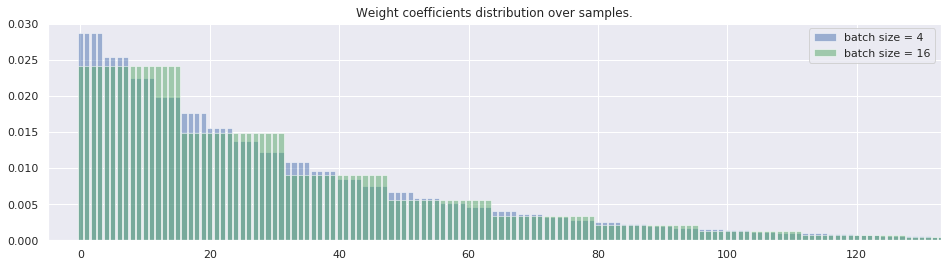
\includegraphics[width=16cm,keepaspectratio=true]{images/momentum_weigth_coefficients.png}
	\caption{
		Weight coefficients with which each sample gradient
		$g_i$
		contributes to a training step under the condition
		\eqref{Formula: m^1/b = m^1/b}.
		The batch sizes are $4$ and $16$, and
		$\sqrt[b]{m} = \sqrt[\tilde b]{\tilde m} = 0.03$.
		The x-axis corresponds to the reverse sample counting.
		The weight coefficient values are visually combined into blocks of sizes
		$b=4$
		or
		$\tilde b = 16$
		depending on the batch size.
		The image illustrates that, despite different batch sizes,
		the momentum can be tuned so that the weight coefficients are close in value.
	}
	\label{Fig: momentum weight coefficients}
\end{figure}

\emph{
	The ultimate goal of our gradient descent hyperparameter reparameterization
	is to separate the technical part related to data parallelism
	from the real smoothing between gradients during the minima search.
}
This motivates an alternative parameterization for
\eqref{Formula: classic SGD with momentum} as follows:
\begin{equation}
	\begin{aligned}
		\mathbf{v}_n &= e^{-\frac{b}{\beta}}\, \mathbf{v}_{n-1}
		 	+ (1 - e^{-\frac{b}{\beta}})\, \sum_{i:\, t(i) = n} \mathbf{g}_i(\boldsymbol\theta_n) \\
		\boldsymbol\theta_n &=
			\boldsymbol\theta_{n-1} - \lambda\, \mathbf{v}_n
	\end{aligned},\quad
	\beta \geq 0, \quad
	\lambda > 0.
	\label{Formula: SGD with momentum reparameterized}
\end{equation}
The case
$\beta = 0$
corresponds to
$m=0$.
The larger the value of
$\beta$,
the stronger the smoothing.

The advantage of the proposed approach is
that we do not have to change the fine-tuned hyperparameters
$\lambda$
and
$\beta$
when moving to different hardware.
It is enough to set the batch size
$b$
as large as possible
(or until we face convergence stability restrictions from Section
\ref{Section: convergence stability}).
The experimental confirmation is presented in Figure
\ref{Fig: batch size and momentum}.

\begin{figure}
	\centering
	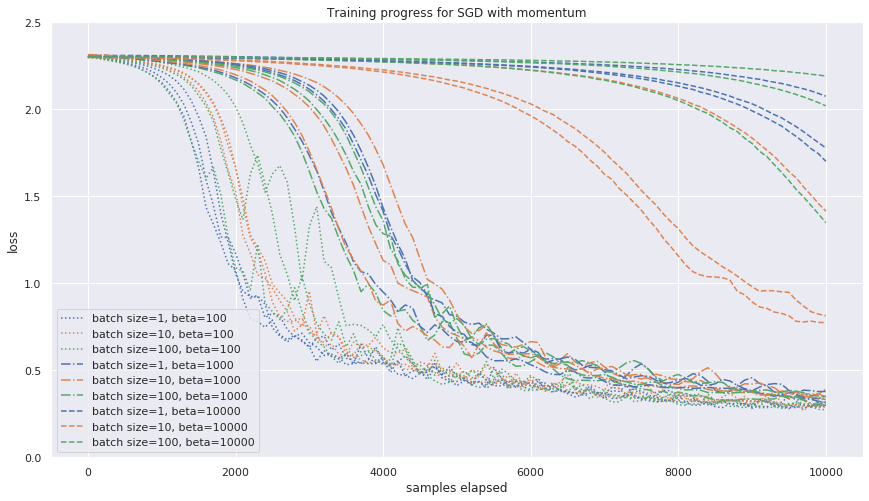
\includegraphics[width=16cm,keepaspectratio=true]{images/batch_size_and_momentum.png}
	\caption{
		Training progress on the MNIST training dataset with various values of the batch size
		$b$
		and
		$\beta$
		from
		\eqref{Formula: SGD with momentum reparameterized}.
		For each pair of
		$b$ and
		$\beta$
		values,
		we sampled 3 experiments,
		demonstrated by 3 corresponding curves of the same color and style.
		It can be observed that batch size change has no visible effect on the loss decay rate with respect to the total number of samples. It is also remarkable that smaller values for the momentum parameter $\beta$ provide faster convergence in our case. This may differ for other problems.
	}
	\label{Fig: batch size and momentum}
\end{figure}

Notice, however, that for
$b \gtrsim \beta$,
the momentum smoothing is weak with respect to ``batch'' smoothing,
and the approximation illustrated in Figure
\ref{Fig: momentum weight coefficients}
is no longer valid.

The relations between the proposed and classic hyperparameter normalization are:
\[\begin{aligned}
	m^{\text{cl}} &= e^{-\frac{b}{\beta}} \\
	\lambda^{\text{cl}} &= \left(1 - e^{-\frac{b}{\beta}} \right) \lambda\, b^{-1}
\end{aligned}\]


\section{Adam Gradient Descent Case}

For other gradient descent methods,
our approach is similar.
For example, Adam gradient descent in its classic parameterization in our notation is:
\begin{equation}
	\begin{aligned}
		\mathbf{v}^{\text{cl}}_n
			&= \beta_1^{\text{cl}}\, \mathbf{v}^{\text{cl}}_{n-1}
			+ (1 - \beta_1^{\text{cl}})\, b^{-1} \sum_{i:~ t(i) = n} \mathbf{g}_i(\boldsymbol\theta_n), \\
		\mathbf{w}^{\text{cl}}_n
			&= \beta_2^{\text{cl}}\, \mathbf{w}^{\text{cl}}_{n-1}
			+ (1 - \beta_2^{\text{cl}})\,
				\left[
					b^{-1} \sum_{i:~ t(i) = n} \mathbf{g}_i(\boldsymbol\theta_n)
				\right]^2, \\
		\boldsymbol\theta_n &=
			\boldsymbol\theta_{n-1} - \alpha^{\text{cl}} \frac
				{\mathbf{m}^{\text{cl}}_n}
				{\sqrt{\mathbf{v}^{\text{cl}}_n} + \varepsilon^{\text{cl}}}, \\
		&0 \leq \beta_1^{\text{cl}} <1, \quad
		0 \leq \beta_2^{\text{cl}} <1, \quad
		\alpha^{\text{cl}} > 0, \quad
		\varepsilon^{\text{cl}} > 0,
	\end{aligned}
	\label{Formula: Adam SGD}
\end{equation}
where the square and square root operations of a vector are elementwise.
We propose the normalization:
\[\begin{aligned}
	\mathbf{v}_n
		&= e^{-\frac{b}{\beta_1}}\, \mathbf{v}_{n-1}
		+ (1 - e^{-\frac{b}{\beta_1}})\, \sum_{i:~ t(i) = n} \mathbf{g}_i(w_n), \\
	\mathbf{w}_n
		&= e^{-\frac{b}{\beta_2}}\, \mathbf{w}_{n-1}
		+ (1 - e^{-\frac{b}{\beta_2}})\,
			\sum_{i:~ t(i) = n} \mathbf{g}_i(w_n)^2, \\
	\boldsymbol\theta_n &=
		\boldsymbol\theta_{n-1} - \alpha \frac
			{\mathbf{v}_n}
			{\sqrt{\mathbf{w}_n} + b\, \varepsilon}, \\
	& 0 \leq \beta_1, \quad
	0 \leq \beta_2, \quad
	\alpha > 0, \quad
	\varepsilon > 0,
\end{aligned}\]
where we deviate slightly from the original Adam algorithm
and replace the square of the gradient sum with the sum of gradient squares across the batch.
It can be empirically checked that the typical values of
$(\sum g)^2$
and
$\sum g^2$
are of the same order of magnitude
At least for the considered MNIST model, typical values of
$\sum g^2$
are approximately two times smaller than
$(\sum g)^2$.

Ignoring the last remark, the relations between the proposed and the classic normalizations are:
\begin{equation}
	\begin{aligned}
		\beta_1^{\text{cl}} &= e^{-\frac{b}{\beta_1}}, \\
		\beta_2^{\text{cl}} &= e^{-\frac{b}{\beta_2}}, \\
		\alpha^{\text{cl}} &= \alpha, \\
		\varepsilon^{\text{cl}} &= b\,\varepsilon.
	\end{aligned}
	\label{Formula: Adam hyperparameter relation}
\end{equation}


\section{Gradient Accumulation Technique}

The relationship between momentum and batch size discussed above is quite straightforward.
However, there is a widely used technique called
\href{https://towardsdatascience.com/what-is-gradient-accumulation-in-deep-learning-ec034122cfa}
{gradient accumulation}.
According to this approach,
we sum up gradients from several batches obtained for the same weight value.
This way, the actual batch size can be increased infinitely, and GRAM is no longer a restriction.

As we saw in section
\ref{Section: convergence stability},
for zero momentum, a higher batch size with a fixed
$\lambda$
can only disrupt the training process.
For momentum training where
$\beta \gtrsim b$,
the batch size change is indistinguishable from a
$\beta$
shift as observed in section
\ref{Section: Gradient descent with momentum}.
Of course, the gradient accumulation trick can provide better results in practice,
but it seems redundant.


\section{Conclusion}

We suggest a strategy to fine-tune the gradient descent hyperparameters as follows.
Use first the hyperparameter normalization as described above, for example, in
\eqref{Formula: Adam hyperparameter relation}.
As a result of this, we can control the convergence rate while changing the batch size.
However, it may happen that following the increase of the batch size,
the convergence stability may be lost.
In this case, we can either reduce
$\lambda$
to restore convergence or refrain from changing the batch size.
The second option has the advantage of faster convergence
with respect to the total calculation cost.

Remark that we did not consider the batch normalization technique here.
This requires additional study because, for different batch sizes,
we have different gradient fluctuation intensities
that impact the final minimum generalization ability.
See, for example,
\href{https://arxiv.org/pdf/1802.06455.pdf}{Mattias Teye, Hossein Azizpour, Kevin Smith}.





%\section{Phrases}
%
%...
%
%Both the gradient accumulation technique
%and strong momentum in stochastic gradient descent with fixed GPU memory batch size
%are dedicated to make the learning process less noisy and more efficient.
%We consider how much they are equivalent in this post.
%
%...
%
%The main thesis of this paper: 
%``batch-size change is approximately equivalent to a certain change of learning rate and momentum''
%
%...
%
%This statement may sounds obvious. However, ...
%
%...
%
%This statement is pretty obvious for some people and not understood for othe
%
%...
%
%
%$$
%	\Delta \mathbf{w} = - \lambda \sum_{i\in\text{min-batch}} \frac{\partial}{\partial \mathbf{w}} L(x_i, y_i; w),
%$$
%where we used a sum over samples in mini-batch bit not the mean value. 
%There relation with the classic normalization is as follows. 
%$\lambda = \frac{\lambda_{\text{classic}}}{N_{\text{mini-batch size}}}$.
%
%...
%
%Let $n$ be a weight update step and let $i$ be a sample number.
%
%...
%
%Let 
%$i = 0, 1, 2, \dotso$
%be the ordering with which the data-label pair 
%$(x_i, y_i)$
%is feeded to the model. 
%Let also
%$t(i)$
%takes values in 
%$\{0, 1, 2 ,\dotso \}$
%
%
%
%...
%
%$$
%	\lambda \sum_i g_i(w)
%$$
%
%
%
%$$
%	\lambda \sum_i g_{i} \left( w_{n(i)} \right) 
%	\approx 
%	\lambda  \sum_i g_{i} \left( w_{\tilde n(i)} \right) 
%$$
%
%
%
%... because the change of 
%
%$g$
%at different points 
%$w$
%can be ignored due to small weight updates.
%
%...




\end{document}






























